\chapter{Introduction}

Density functional theory (DFT) is a field in physics which is commonly applied in the fields of quantum chemistry,
solid state physics and material sciences. It is based on the Hohenberg-Kohn theorems \cite{hohenberg_inhomogeneous_1964} which state that the ground-state properties of a many-electron system are uniquely determined by its electron density.

Based on these insigths Kohn Sham theory was conceived, which strives to reproduce the ground state
density of a complex many-body quantum mechanical system with a set of non-interacting particles which are govered by the much simpler Kohn Sham equation. The non interacting electrons are represented by so called orbitals $\{\phi_i (\mathbf{r})\}_{i=1,...,n}$, which are pairwise orthogonal and normalized. They combine to form the density of the system $\rho(\mathbf{r}) = || \sum\limits_{i=1}^N \phi_i(\mathbf{r})||^2$.

\begin{align}
    H_{KS}[\rho ]  = T_S [\rho] + V_{eff}[\rho]
\end{align}

Dispite its great success KS-DFT has also some short commings. By using orbitals to describe the system it is bound to computationally scale very poorly to larger system sizes. Its accuracy is also heavily dependent on the choice of the exchange correlation functional which is used to approximate the many body effects of the system and the basis on which the orbitals are defined.

New approaches try to fullfill Hohenberg-Kohn promise of a functional dependendent only on the electron density. These approaches are commonly named the Orbital Free DFT (OFDFT) and while older ones use classical density functionals\cite{oldofdft}, newer ones use machine learning models to approximate the functional.\cite{Roman}\cite{zhang_m-ofdft_2023}.

In both cases well shaped basis sets are neccessary to represent the orbitals of kohn sham or the electron density in OF-DFT. Well optimised basis sets for dft calculation exist for a long time \cite{something} but they mostly use fixed basis functions for every atom type to represent the individual orbitals. In some case adaptive basis functions were used to adapt the local basis function to their local environment \cite{something}. But in these  attemps were mostly complicated by the complex integrals which are nessesary to compute the energy of the system. In this work we introduce differentiable integrals which with the help of machine learning technics and automatic diffentaition are  able to optimize baiss sets in an more effective way than previously employed finite difference methods. These integrals can be used to both optimize the orbtials free as well as the kohn sham basis sets for bath their coefficients as well as their exponents. They can also be used to learn advanced adaptive basis functions which use a graph neural network to adapt the basis functions to their local environment , greatly increasing the accuracy of the dft calculation with very minimal cost.
\newpage
\section{Conventions and Notations}
Here we are going to to summarize the conventions that are being followed in this work.
\subsection{Einstein summation}
In this work we are using Einstein summation notation, which is a compact notation for expressing the sum of products of vectors in a vector space. In this notation, summation is implied whenever two indices appear in a product term, one subscript and one superscript. For example, the sum
\begin{align}
    a_i b^i = \sum_{i=1}^n a_i b^i
\end{align}
is implied by the notation. The summation convention is used in this work for all repeated indices, unless otherwise stated.
\subsection{Integral Notation}\label{integral_notation}
We are using Bra-Ket Notation, which is commonly used in quantum mechanics. For two functions $\phi,\psi:\mathbb{R}^3\rightarrow \mathbb{C}$
\begin{align}
    \langle \phi | \psi\rangle &:= \int \phi(\mathbf r)\psi^\dagger(\mathbf r) d\mathbf r
\end{align}
As we are mostly interested in the ground state, which can be described by purely real functions, we can omit the dagger in the notation.
We also note hartree integrals by round brackets, for example
\begin{align}
    (\phi | \psi) &:= \int \int \frac{\phi(\mathbf r)\psi^\dagger(\mathbf r')}{|\mathbf{r}-\mathbf{r'}|} d\mathbf rd\mathbf {r'}
\end{align}
\subsection{Data visualization}\label{boxplots}
To visualize distributions boxplots can give a good overview over the underlying statistics without overcrowding the plotwith to many information. The following visual guide demonstates how the plots used in the work are ment to be interpreted.
\begin{figure}[H]
    \centering
    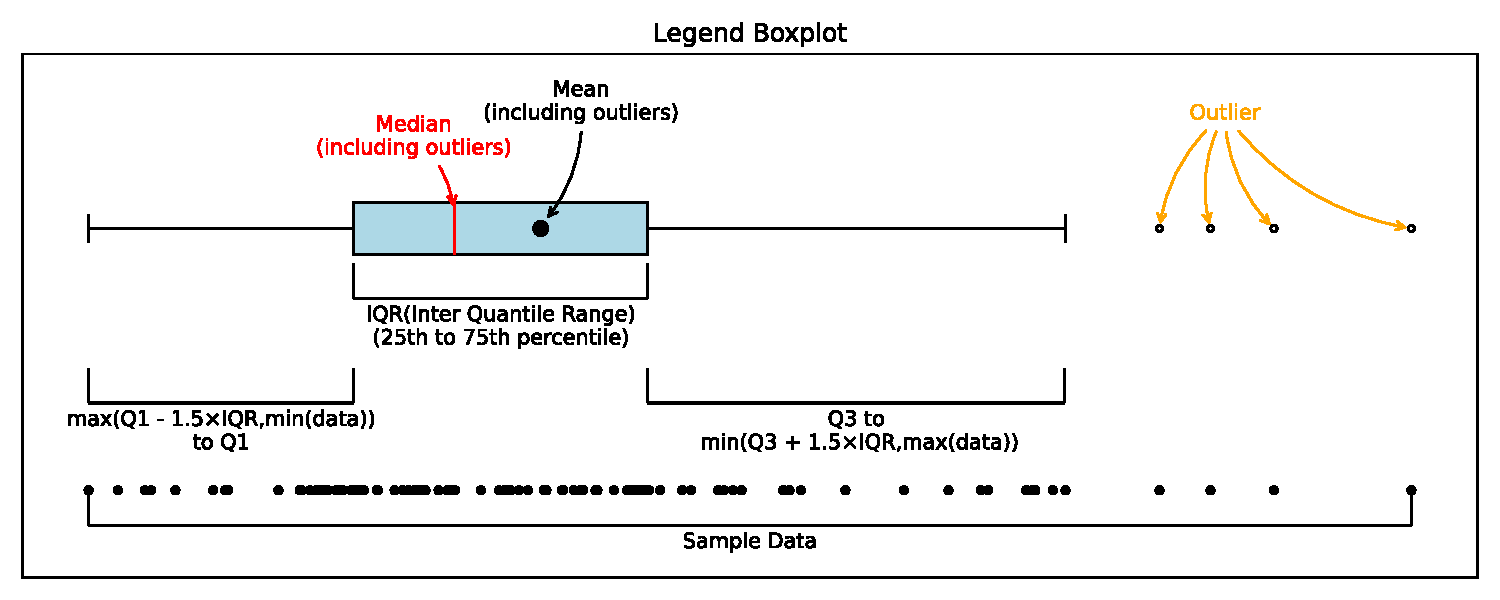
\includegraphics[width=1.\textwidth]{chapters/foundations/images_foundation/legend_boxplot}
    \caption{A boxplot showing the distribution of a toy data set with the important features labeled. Note that the left whiskers is shorted, which indicates that the data is right skewed.}
\end{figure}
Another challenge is the visualisation of the electron density of a molecule. In this work we are